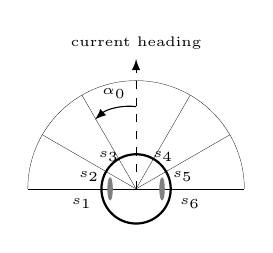
\begin{tikzpicture}[scale=0.55,font=\tiny]

% sensors
\draw [ultra thin, rotate=0](0,0) --  (2.5,0) node[midway, below]{$s_6$};
\draw [ultra thin, rotate=30](0,0) --  (2.5,0) node[midway, below]{$s_5$};;
\draw [ultra thin, rotate=60](0,0) --  (2.5,0) node[midway, below]{$s_4$};;
\draw [ultra thin, rotate=120](0,0) --  (2.5,0) node[midway, below]{$s_3$};;
\draw [ultra thin, rotate=150](0,0) --  (2.5,0) node[midway, below]{$s_2$};;
\draw [ultra thin, rotate=180](0,0) --  (2.5,0) node[midway, below]{$s_1$};;
% angle
\draw [-latex](0,1.9) arc (82.9738:132:1.2) node[midway,above]{$\alpha_0$};
\draw [dashed,-latex](0,0) --  (0,3) node[at end, above]{current heading};
% robot
\draw [thick] (0,0) ellipse (0.8 and 0.8);
% wheels
\draw  [fill,gray, rotate around={90:(0.6,0)} ]  (0.6,0) node (v1) {} ellipse (0.25 and 0.05);
\draw  [fill,gray, rotate around={90:(-0.6,0)} ]  (-0.6,0) node (v2) {} ellipse (0.25 and 0.05);
% circle
\draw [ultra thin] (2.5,0) arc (0:180:2.5);

\end{tikzpicture}